\documentclass{article}
\usepackage[utf8]{inputenc}
\usepackage{graphicx}
\usepackage{epstopdf}
\usepackage{float}
\usepackage[margin=1.25in]{geometry}
\usepackage{amsmath}
\usepackage{amssymb}
\usepackage{color} 
\usepackage{fancyvrb} 
\newcommand{\Vout}{{$V_{out}$}}
\newcommand{\Vb}{{$V_{b}$}}
\newcommand{\Vcm}{{$V_{cm}$}}
\newcommand{\Vdm}{{$V_{dm}$}}
\newcommand{\Vtwo}{{$V_{2}$}}
\newcommand{\Vone}{{$V_{1}$}}
\newcommand{\Itwo}{{$I_{2}$}}
\newcommand{\Ione}{{$I_{1}$}}
\newcommand{\Vdd}{{$V_{dd}$}}
\newcommand{\Iout}{{$I_{out}$}}
\newcommand{\Vin}{{$V_{in}$}}
\newcommand{\gm}{{$g_{m}$}}
\newcommand{\Idm}{{$I_{dm}$}}
\newcommand{\Icm}{{$I_{cm}$}}
\newcommand{\Ib}{{$I_{b}$}}
\newcommand{\nMOS}{{\textit{n}MOS }}
\newcommand{\pMOS}{{\textit{p}MOS }}
\newcommand{\Mone}{{$M_{1}$}}
\newcommand{\Mtwo}{{$M_{2}$}}
\newcommand{\Mthree}{{$M_{3}$}}
\newcommand{\Mfour}{{$M_{4}$}}
\newcommand{\Mb}{{$M_{b}$}}
\title{Circuits Lab 8}
\author{Cory Dolphin and Noam Rubin}
\date{\today}

\begin{document}

\maketitle

\begin{figure}[H]
\centering
\includegraphics[width=0.6\linewidth]{../Figures/Lab8Schematic}
\caption{A schematic of the differential amplifier used in this lab, with some extra voltages and currents annotated for the purpose of analysis.}
\label{fig:lab8schem}
\end{figure}


\section*{Experiment 1}
We began by building a simple differential amplifier from an \nMOS differential pair and a \pMOS current mirror. We set the bias transistor just at threshold by applying a bias voltage of $V_B=0.6V$ We connected both inputs together such that the differential mode voltage was zero, and swept the common mode voltage from $+5V$ to $0V$, measuring the output voltage, \Vout. 
A plot of \Vout as a function of \Vcm can be seen below in Figure \ref{fig:exp1p1}. For values of \Vcm greater than the bias voltage, $0.6V$, \Vout appears to change very little with large changes in \Vcm.  We determined the common-mode gain of the amplifier by applying a linear fit to the data. The linear fit found had a slope $-0.202$. Notably, the output voltage appeared to stabilize at approximately $4.3V$.
Though we expected a negative common-mode gain on the order of a few percent, our gain is larger than expected, because XXXXXXXXXXX.

\begin{figure}[H]
\centering
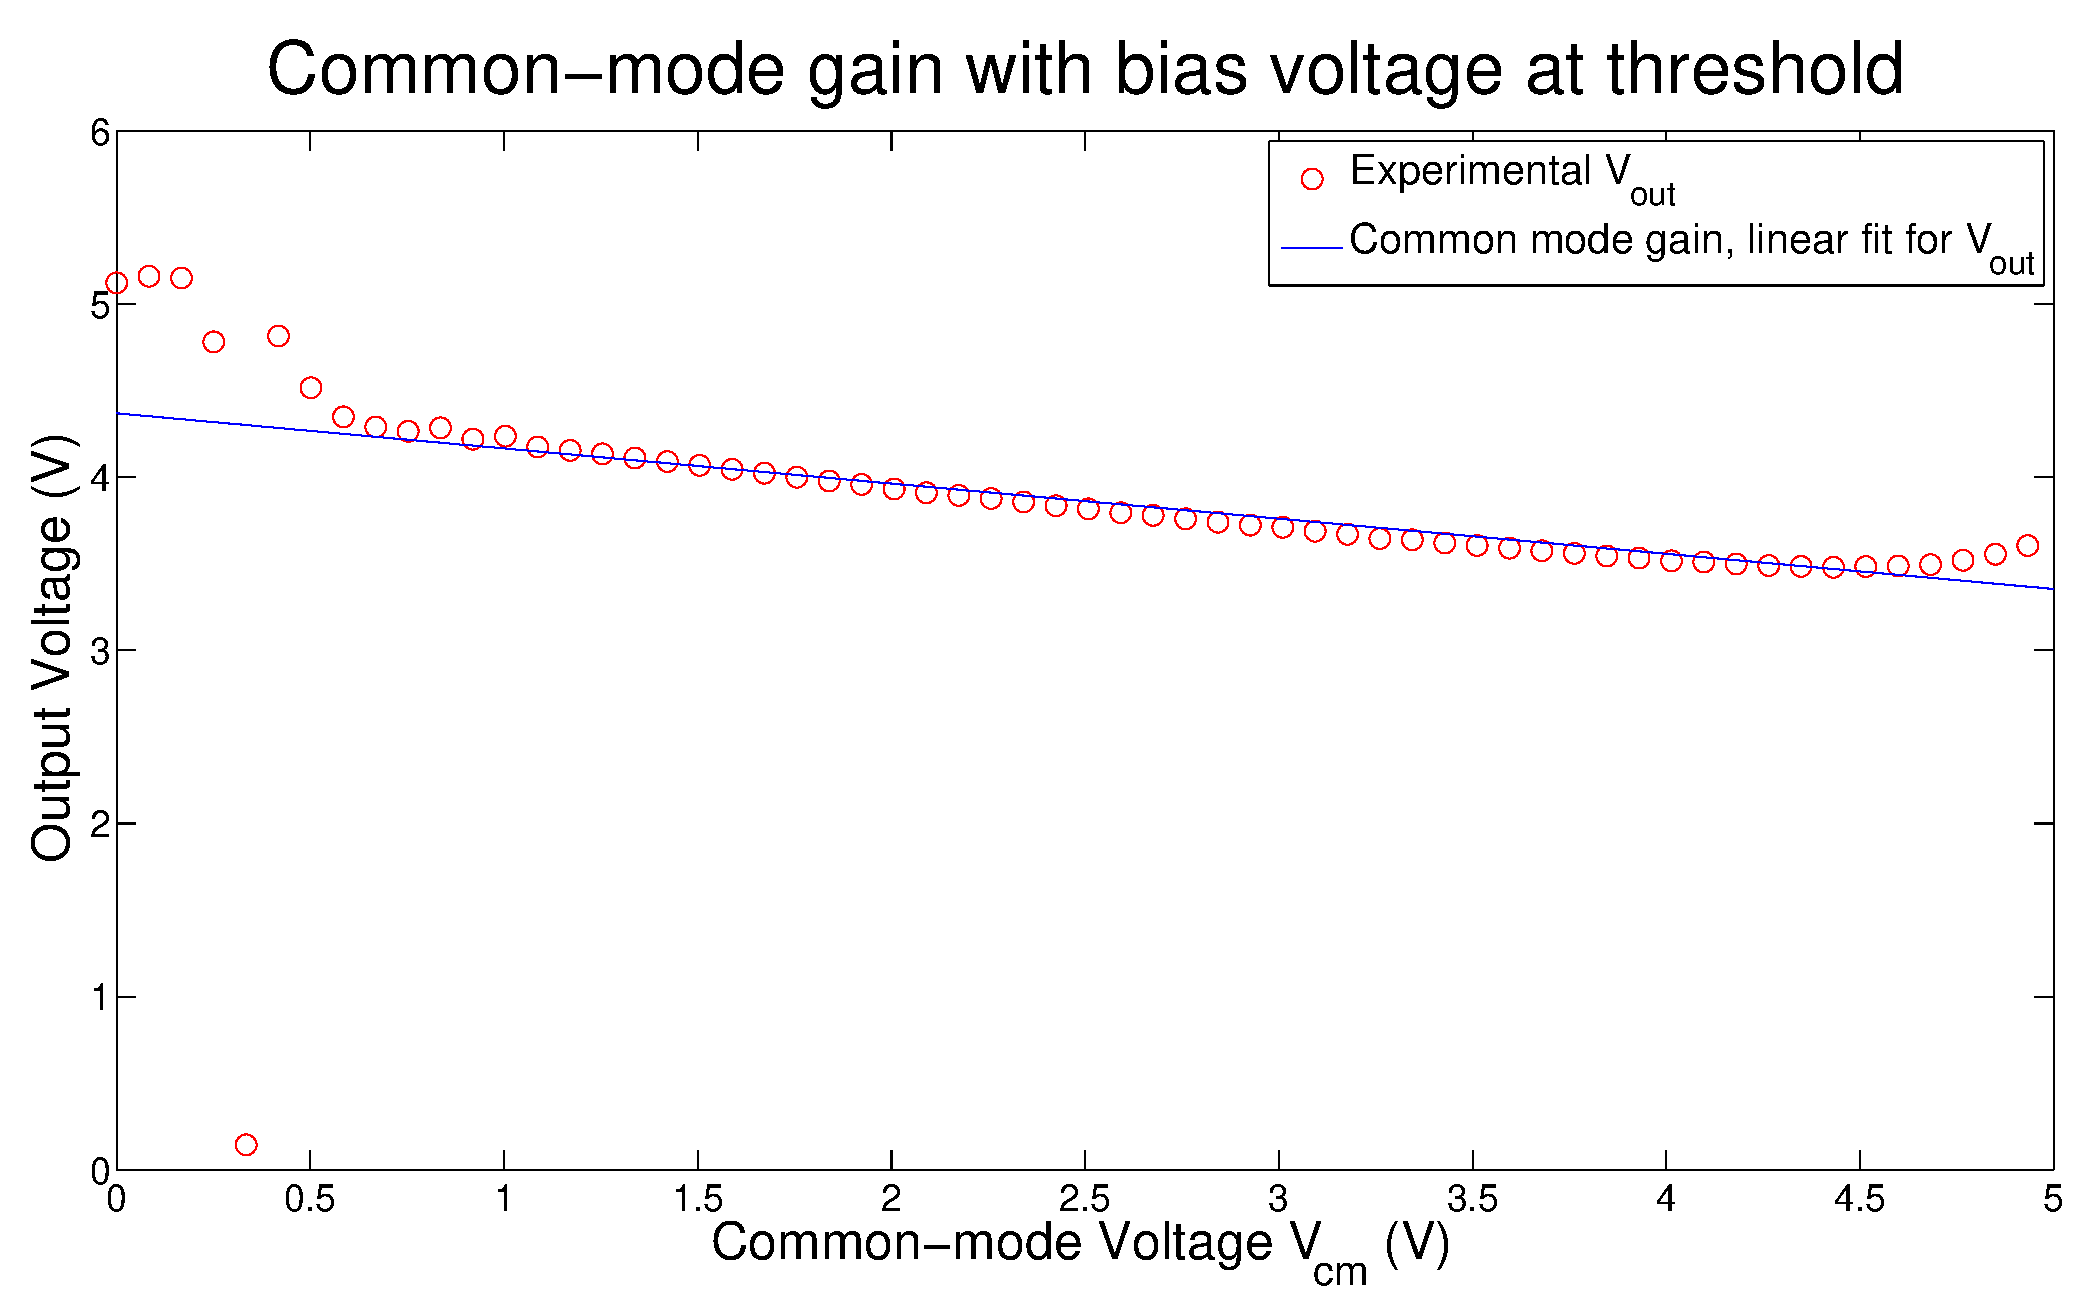
\includegraphics[width=\linewidth]{../Figures/Exp1P1.eps}
\caption{For values of \Vcm greater than the bias voltage, $0.6V$, \Vout appears to change very little with large changes in \Vcm.  We determined the common-mode gain of the amplifier by applying a linear fit to the data. The linear fit found had a slope $-0.202$.}
\label{fig:exp1p1}
\end{figure}

We then connected \Vtwo to a constant voltage source and sweep \Vone from one $+5V$ to $0V$, measuring \Vout for \Vtwo set to three different voltages, $2V$, $3V$ and $4V$.

The voltage transfer characteristic for these experiments, shown in Figure \ref{fig:exp1p2} show three major regions of operation: one in which \Vout increases linearly with a small slope relative to \Vone, when \Vone is less than \Vtwo; another in which \Vout rapidly increases to the positive rail over a small voltage range, when \Vone is slightly greater than \Vtwo; and a third, in which \Vout is pinned at the $+5V$ rail.


\begin{figure}[H]
\centering
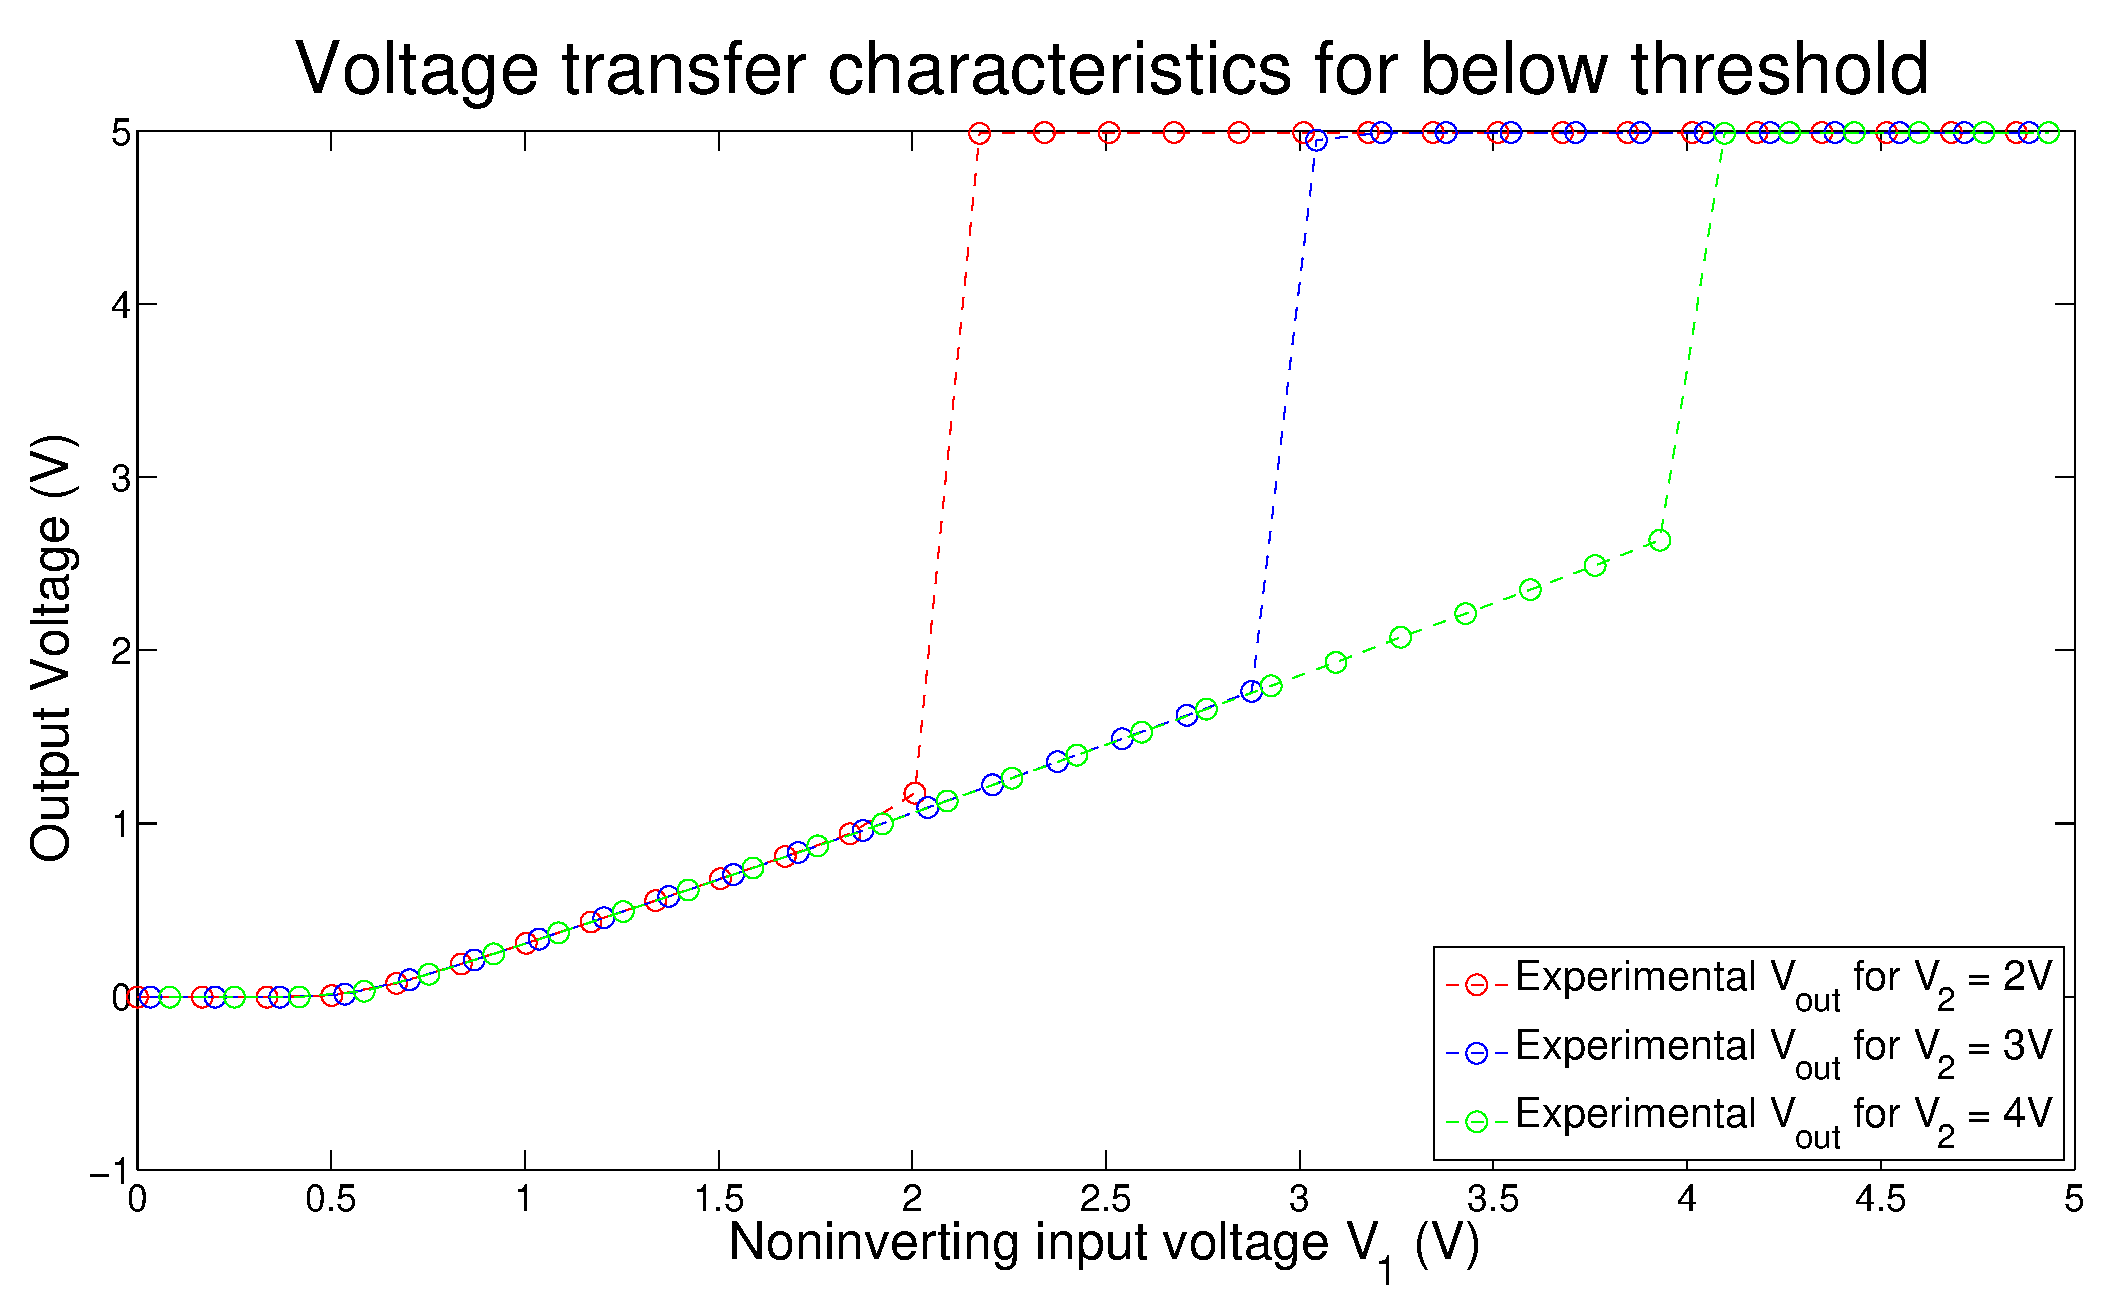
\includegraphics[width=\linewidth]{../Figures/Exp1P2.eps}
\caption{Note that the three series are similar in shape, with the point of inflection equaling the second input voltage for each series.}
\label{fig:exp1p2}
\end{figure}


Repeating the experiment with the bias transistor in strong inversion, with $V_b = 1.5V$, we found a similar pattern to the previous experiment, though the time-scale seemed to be extended.

In the case of the common-mode gain, we found that \Vout ultimately achieved a voltage of roughly $3.8V$, roughly $0.5V$ less than in the weak inversion case. Further, \Vout changed even less relative to \Vcm when \Vcm was greater than \Vb. With the bias transitor strongly inverted, we found a common-mode gain of $-0.039$, a magntidue more similar to the value expected. Meanwhile, for common-mode voltages less than \Vb, \Vout changed far more rapidly.

\begin{figure}[H]
\centering
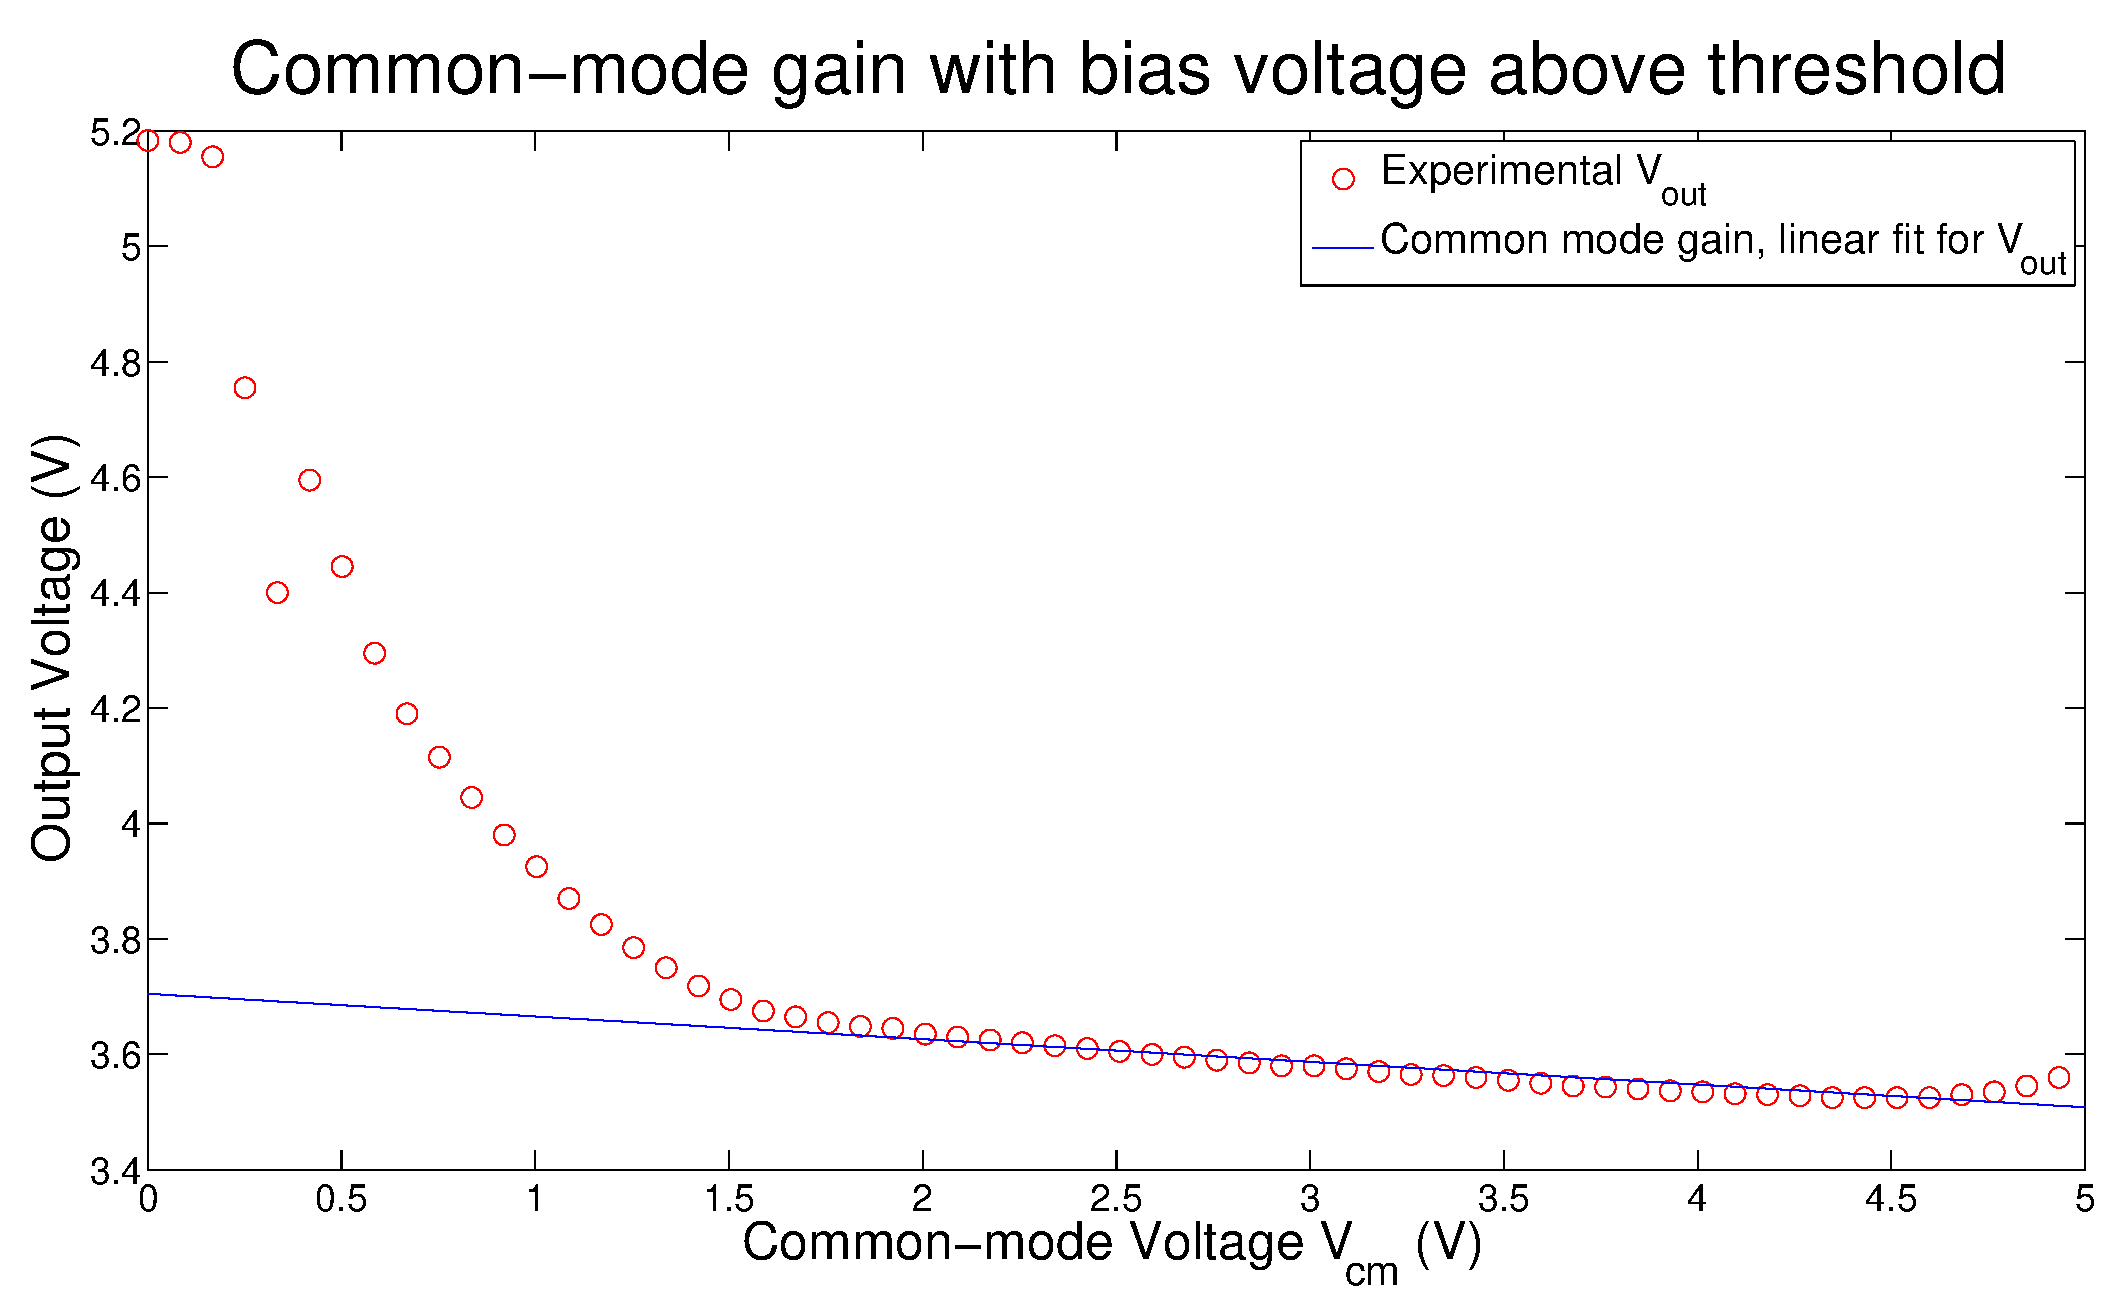
\includegraphics[width=\linewidth]{../Figures/Exp1P4.eps}
\caption{Something descriptive..}
\label{fig:exp1p4}
\end{figure}

When sweeping \Vdm through a range of values, we found that a similar relationship held, three major regions were found on the voltage transfer characteristic shown in Figure \ref{fig:exp1p3}:one in which \Vout increases linearly with a small slope relative to \Vone, when \Vone is less than \Vtwo; another in which \Vout rapidly increases to the positive rail over a small voltage range, when \Vone is slightly greater than \Vtwo; and a third, in which \Vout is pinned at the $+5V$ rail.
One major difference between the behavior with the bias transistor in strong inversion was the rate at which \Vout changed when \Vone increased just past \Vtwo; the output voltage approached the $+5V$ rail more slowly than in the weak inversion case, and appeared to somewhat smooth the discontinuities found in the previous case, linking the three regions with a more sigmoidal shape.

\begin{figure}[H]
\centering
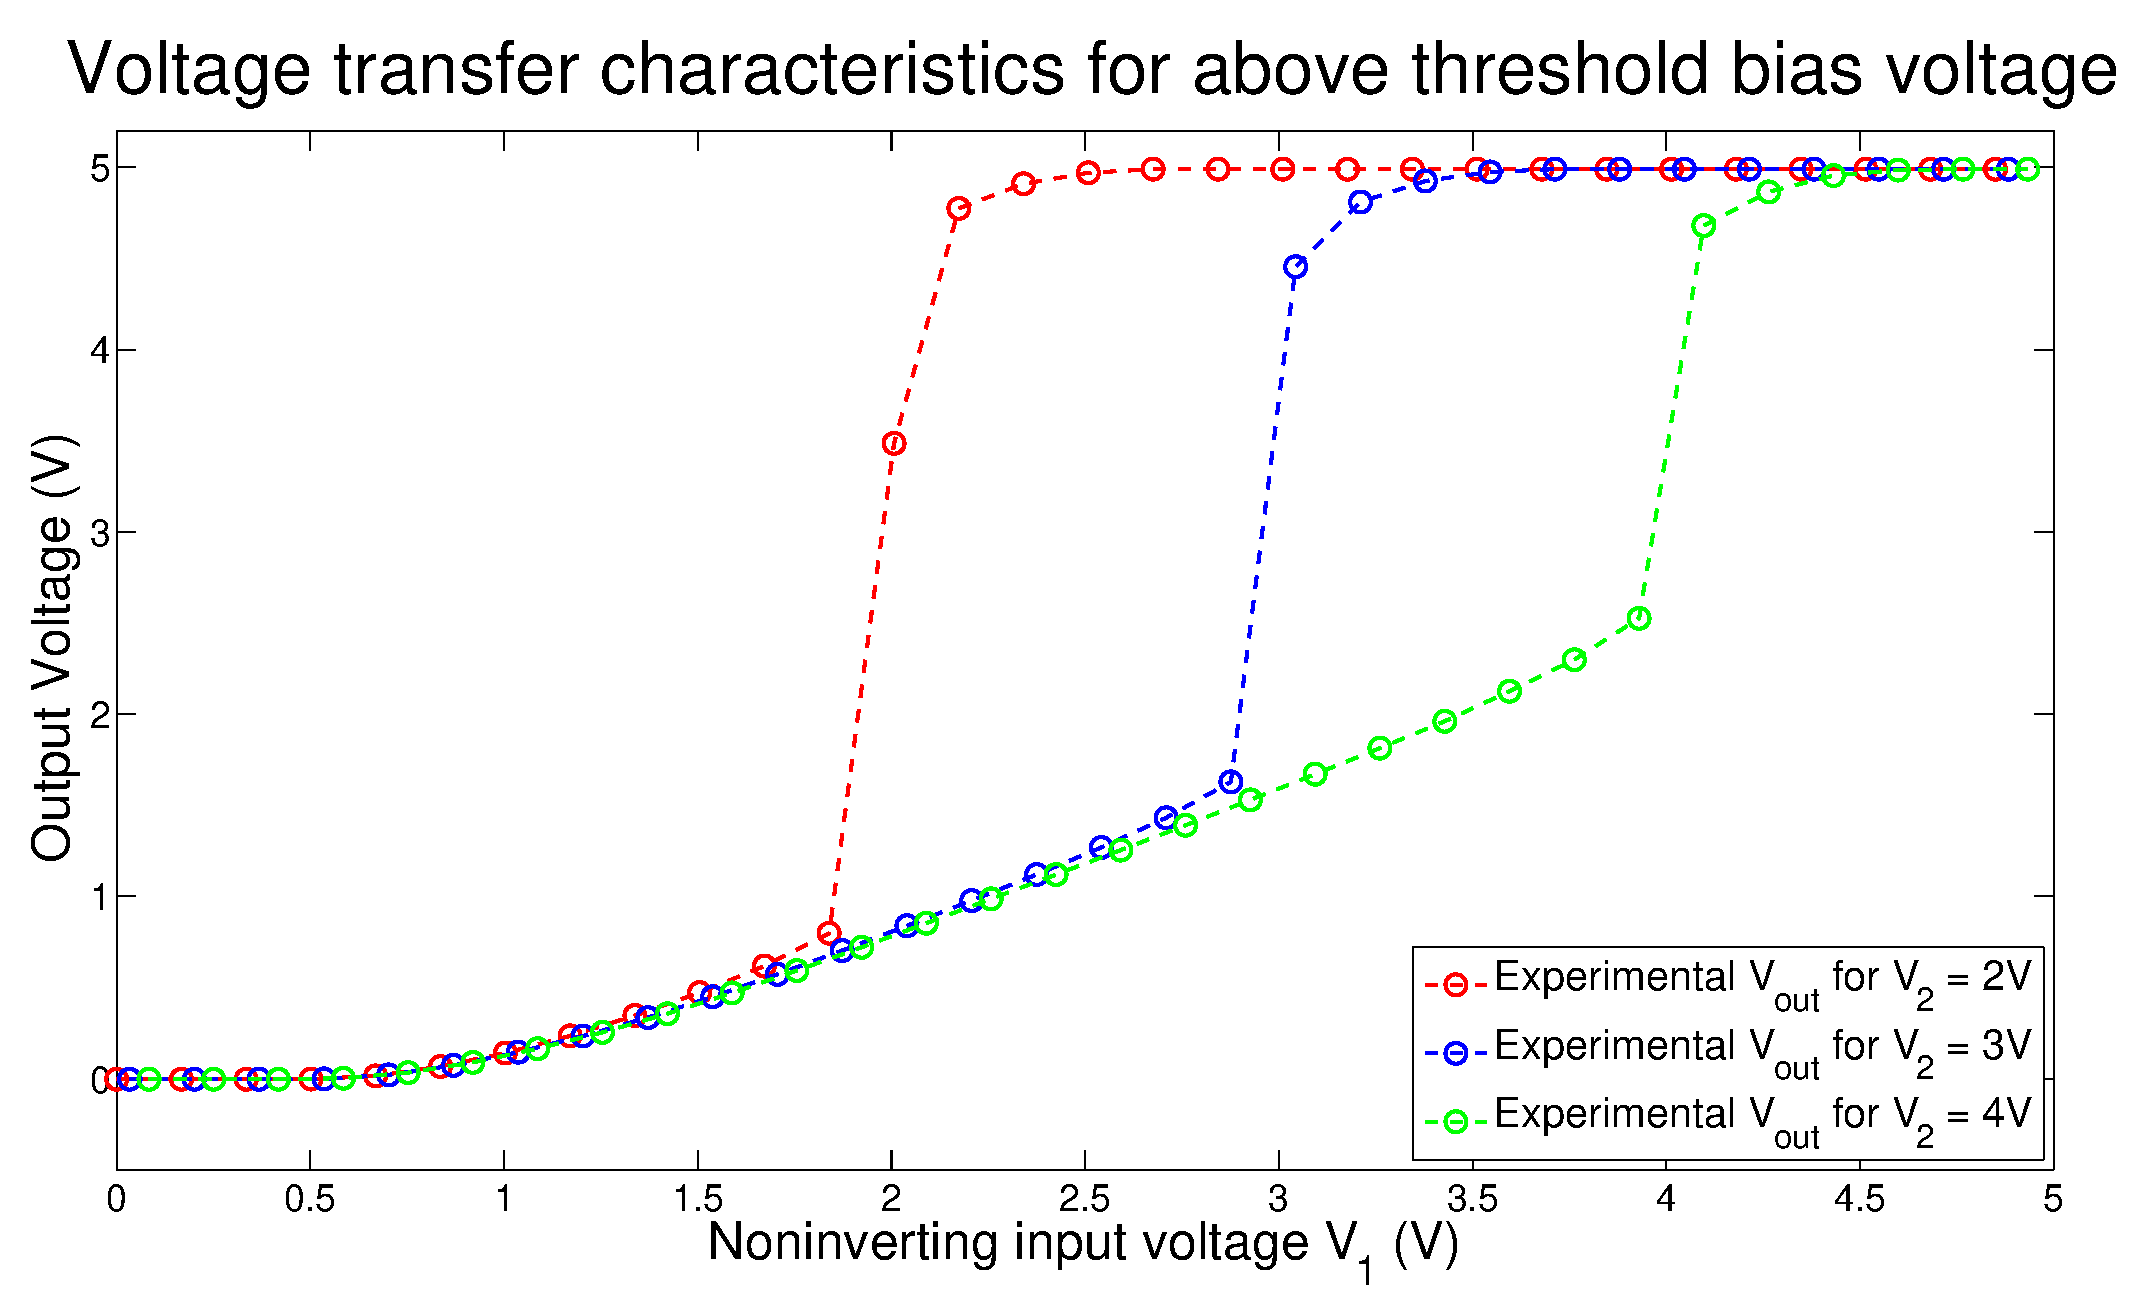
\includegraphics[width=\linewidth]{../Figures/Exp1P3.eps}
\caption{Note that the three series are similar in shape, with the point of inflection equaling the second input voltage for each series.}
\label{fig:exp1p3}
\end{figure}


\textit{Does the behavior of the circuit dffer substantially when biased in strong inversion compared to that which it exhibits in
weak or moderate inversion?}



\section*{Experiment 2}

\begin{figure}[H]
\centering
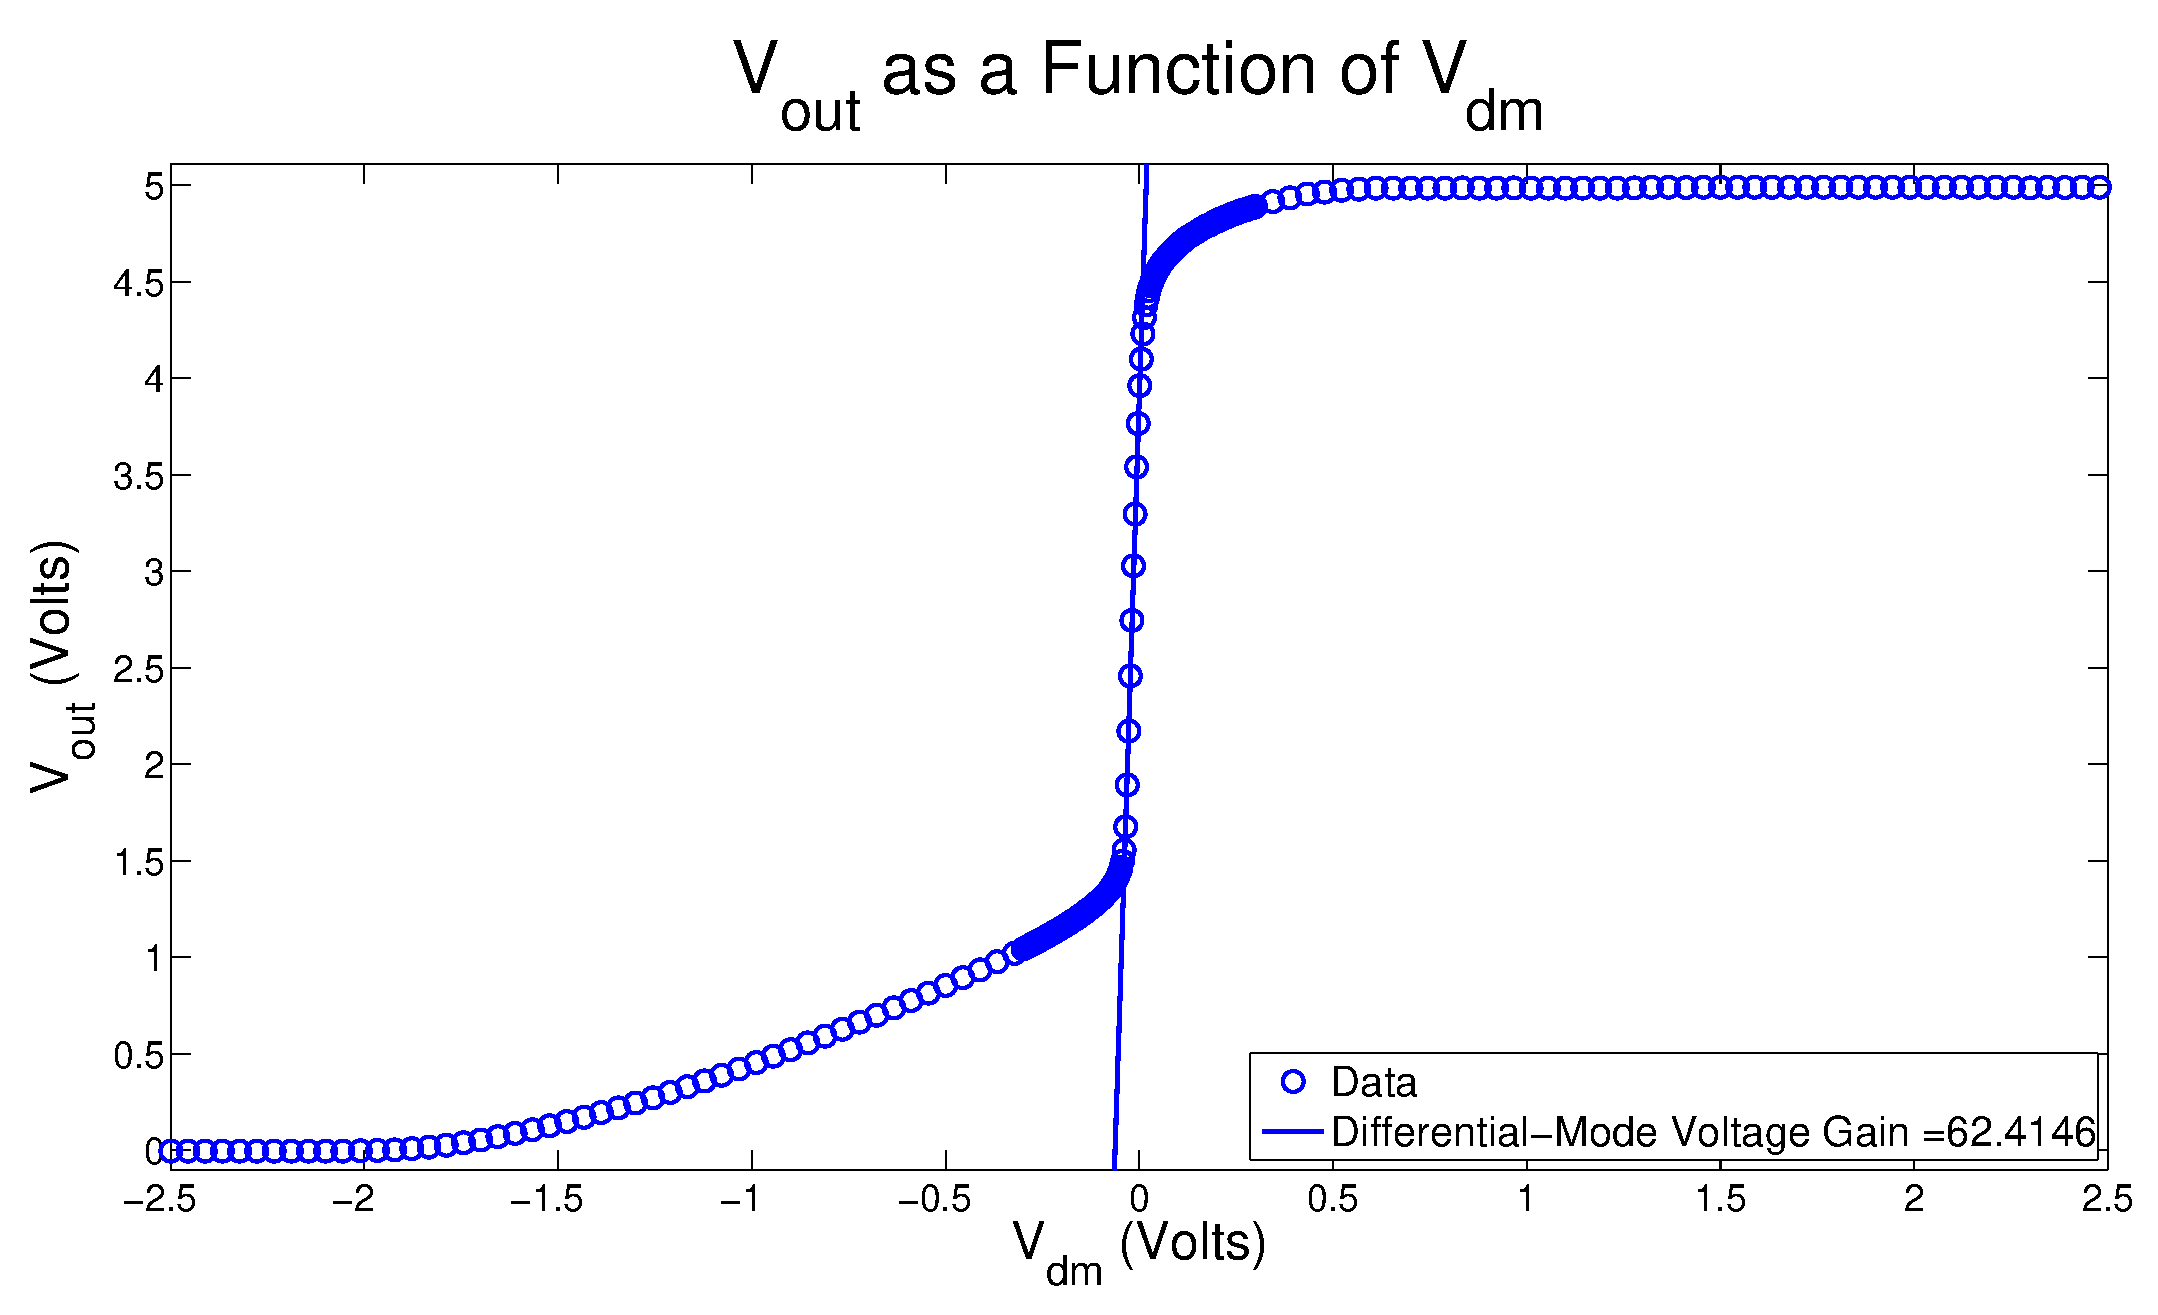
\includegraphics[width=\linewidth]{../Figures/Exp2P1.eps}
\caption{Something descriptive..}
\label{fig:exp2p1}
\end{figure}

\begin{figure}[H]
\centering
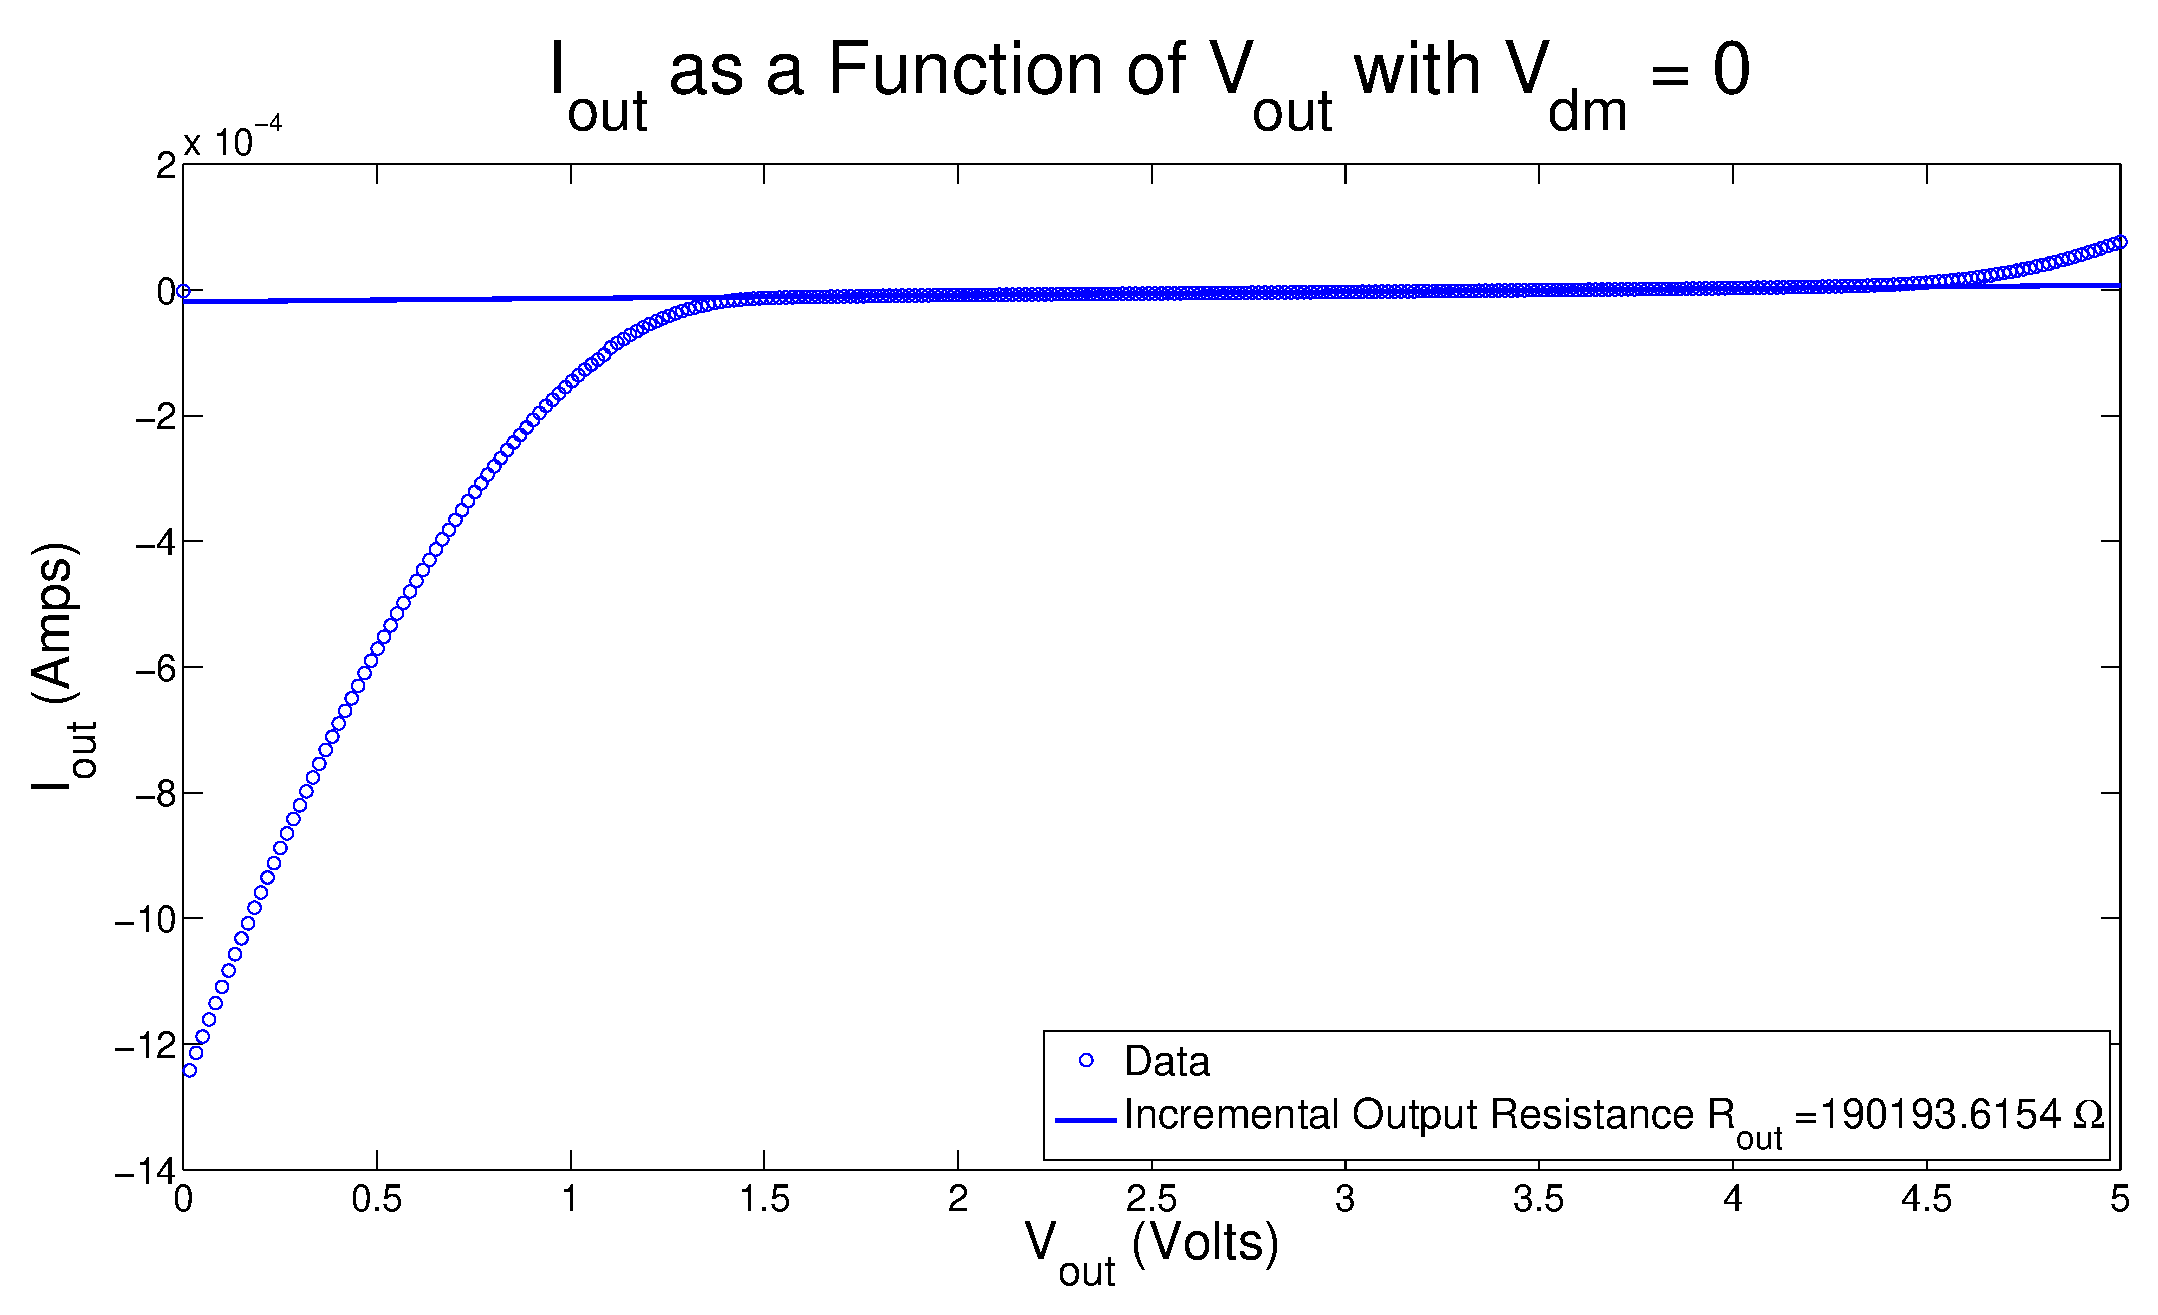
\includegraphics[width=\linewidth]{../Figures/Exp2P2.eps}
\caption{Something descriptive..}
\label{fig:exp2p2}
\end{figure}

\begin{figure}[H]
\centering
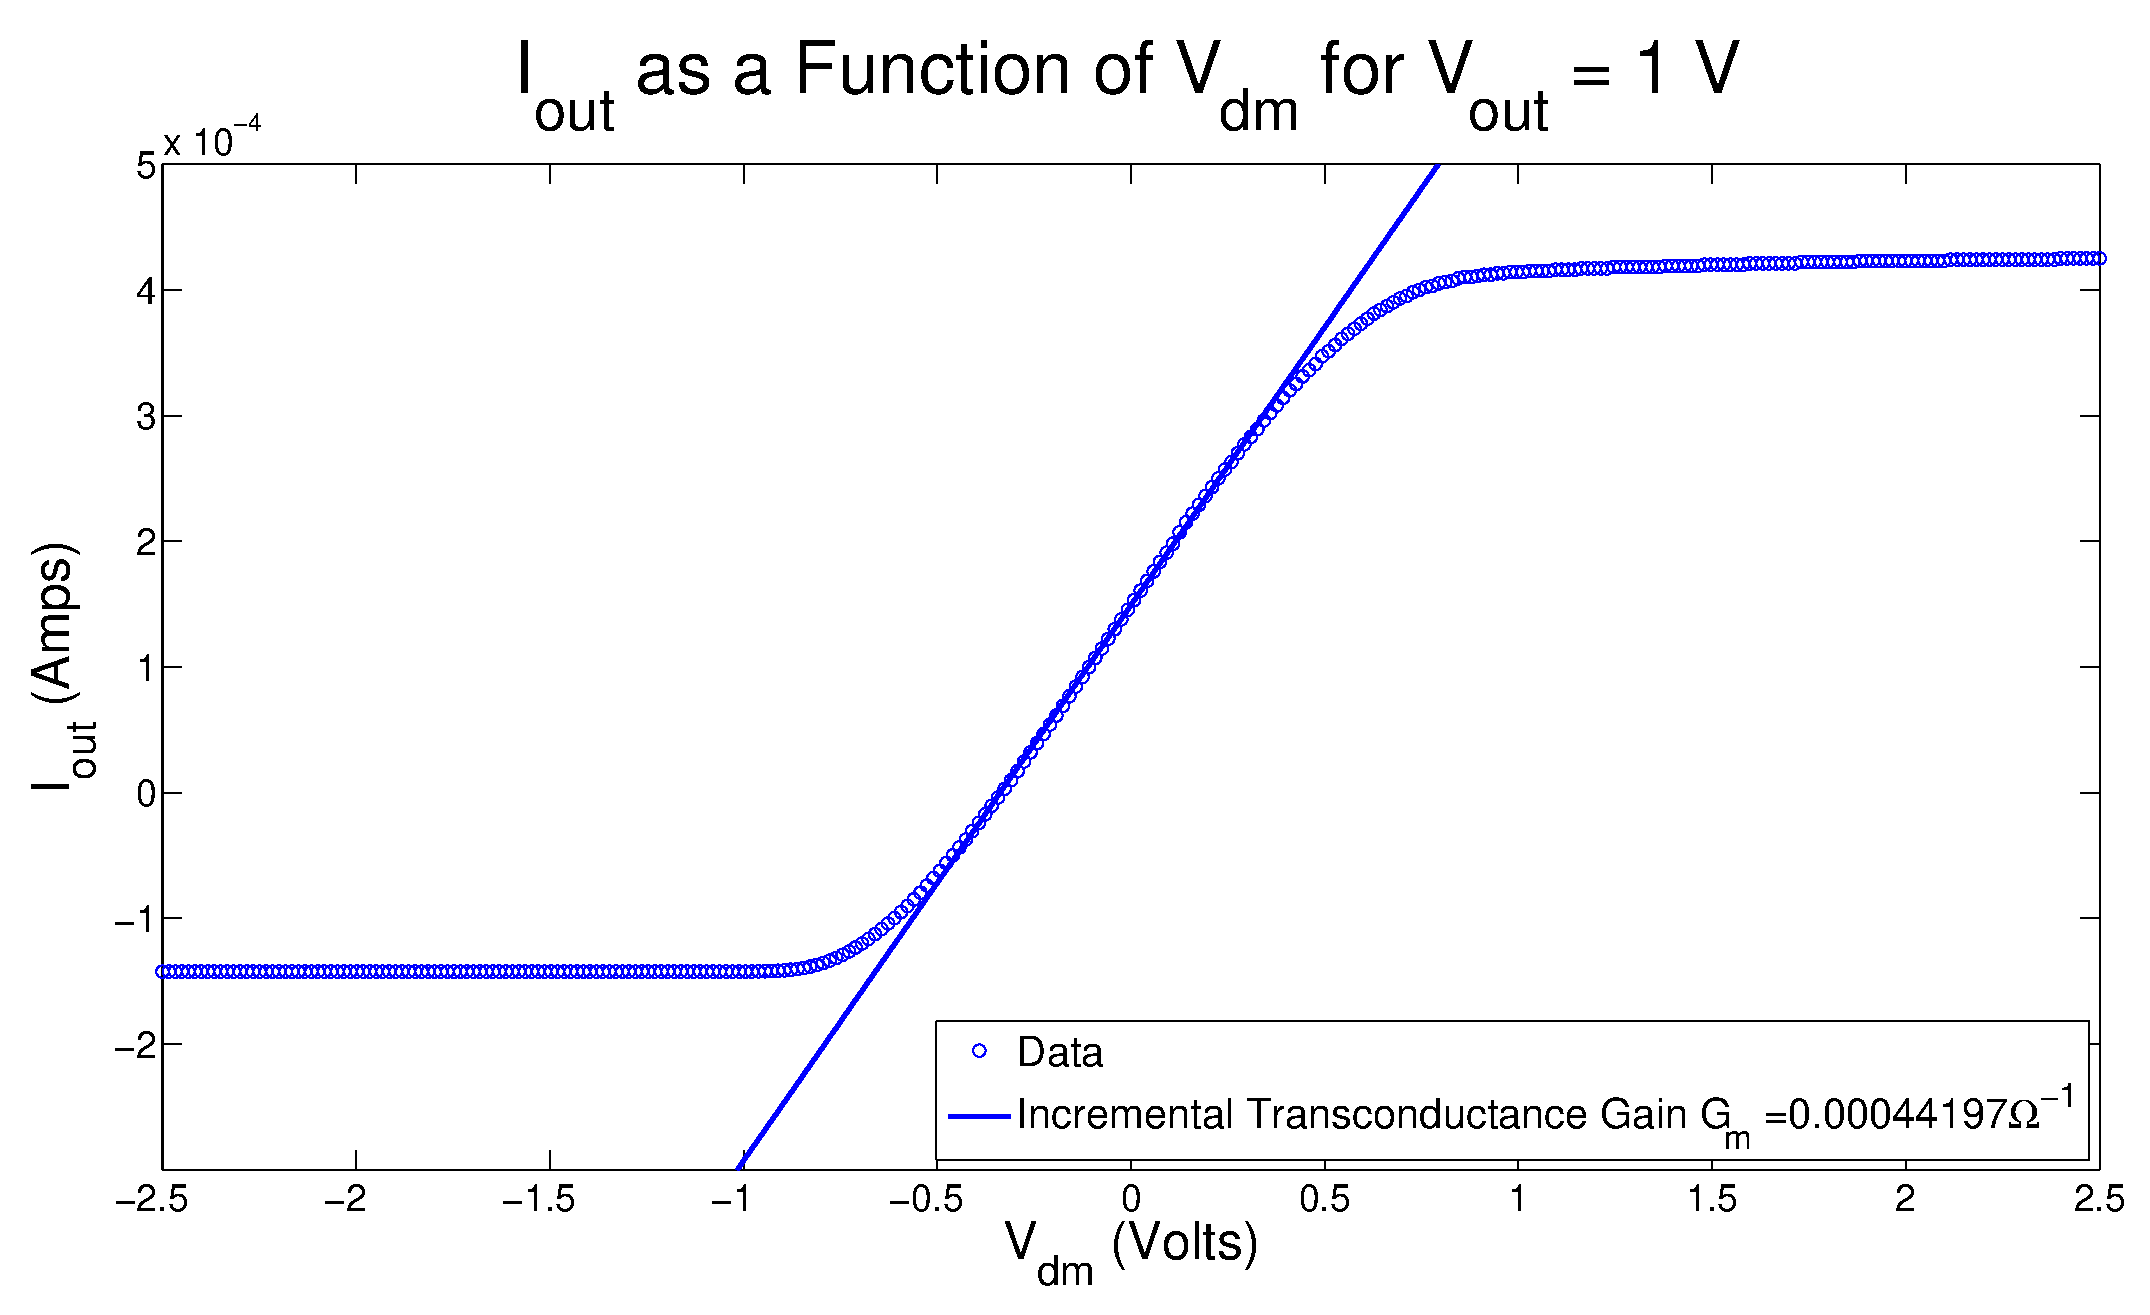
\includegraphics[width=\linewidth]{../Figures/Exp2P3.eps}
\caption{Something descriptive..}
\label{fig:exp2p3}
\end{figure}

\textit{How does this value of for the differential-mode gain compare to that which you obtained directly from the slope of the
VTC? How does the differential-mode voltage gain of the circuit compare to the commonmode voltage gain of the circuit that you found in Experiment 1? Compute a CMRR for the circuit from the ratio of the differential-mode voltage gain to the common-mode voltage
gain that you found in Experiment 1.}


\section*{Experiment 3} 

\textit{Is the incremental gain close to unity?}

\begin{figure}[H]
\centering
\includegraphics[width=0.5\linewidth]{../Figures/Voltage-follower}
\caption{Simple voltage follower we built in Experiment 3.}
\label{fig:voltagefollow}
\end{figure}

The last experiment we conducted involved connecting the inverting input of the differential amplifier, \Vtwo, to the outpout of the differential amplifier, \Vout. We expected the circuit to then behave like a unity-gain voltage follower, as seen in figure \ref{fig:voltagefollow}. In a unity-gain voltage follower, the output follows the non-inverting input, so we expect the ratio between \Vout and \Vin to be 1.

\begin{figure}[H]
\centering
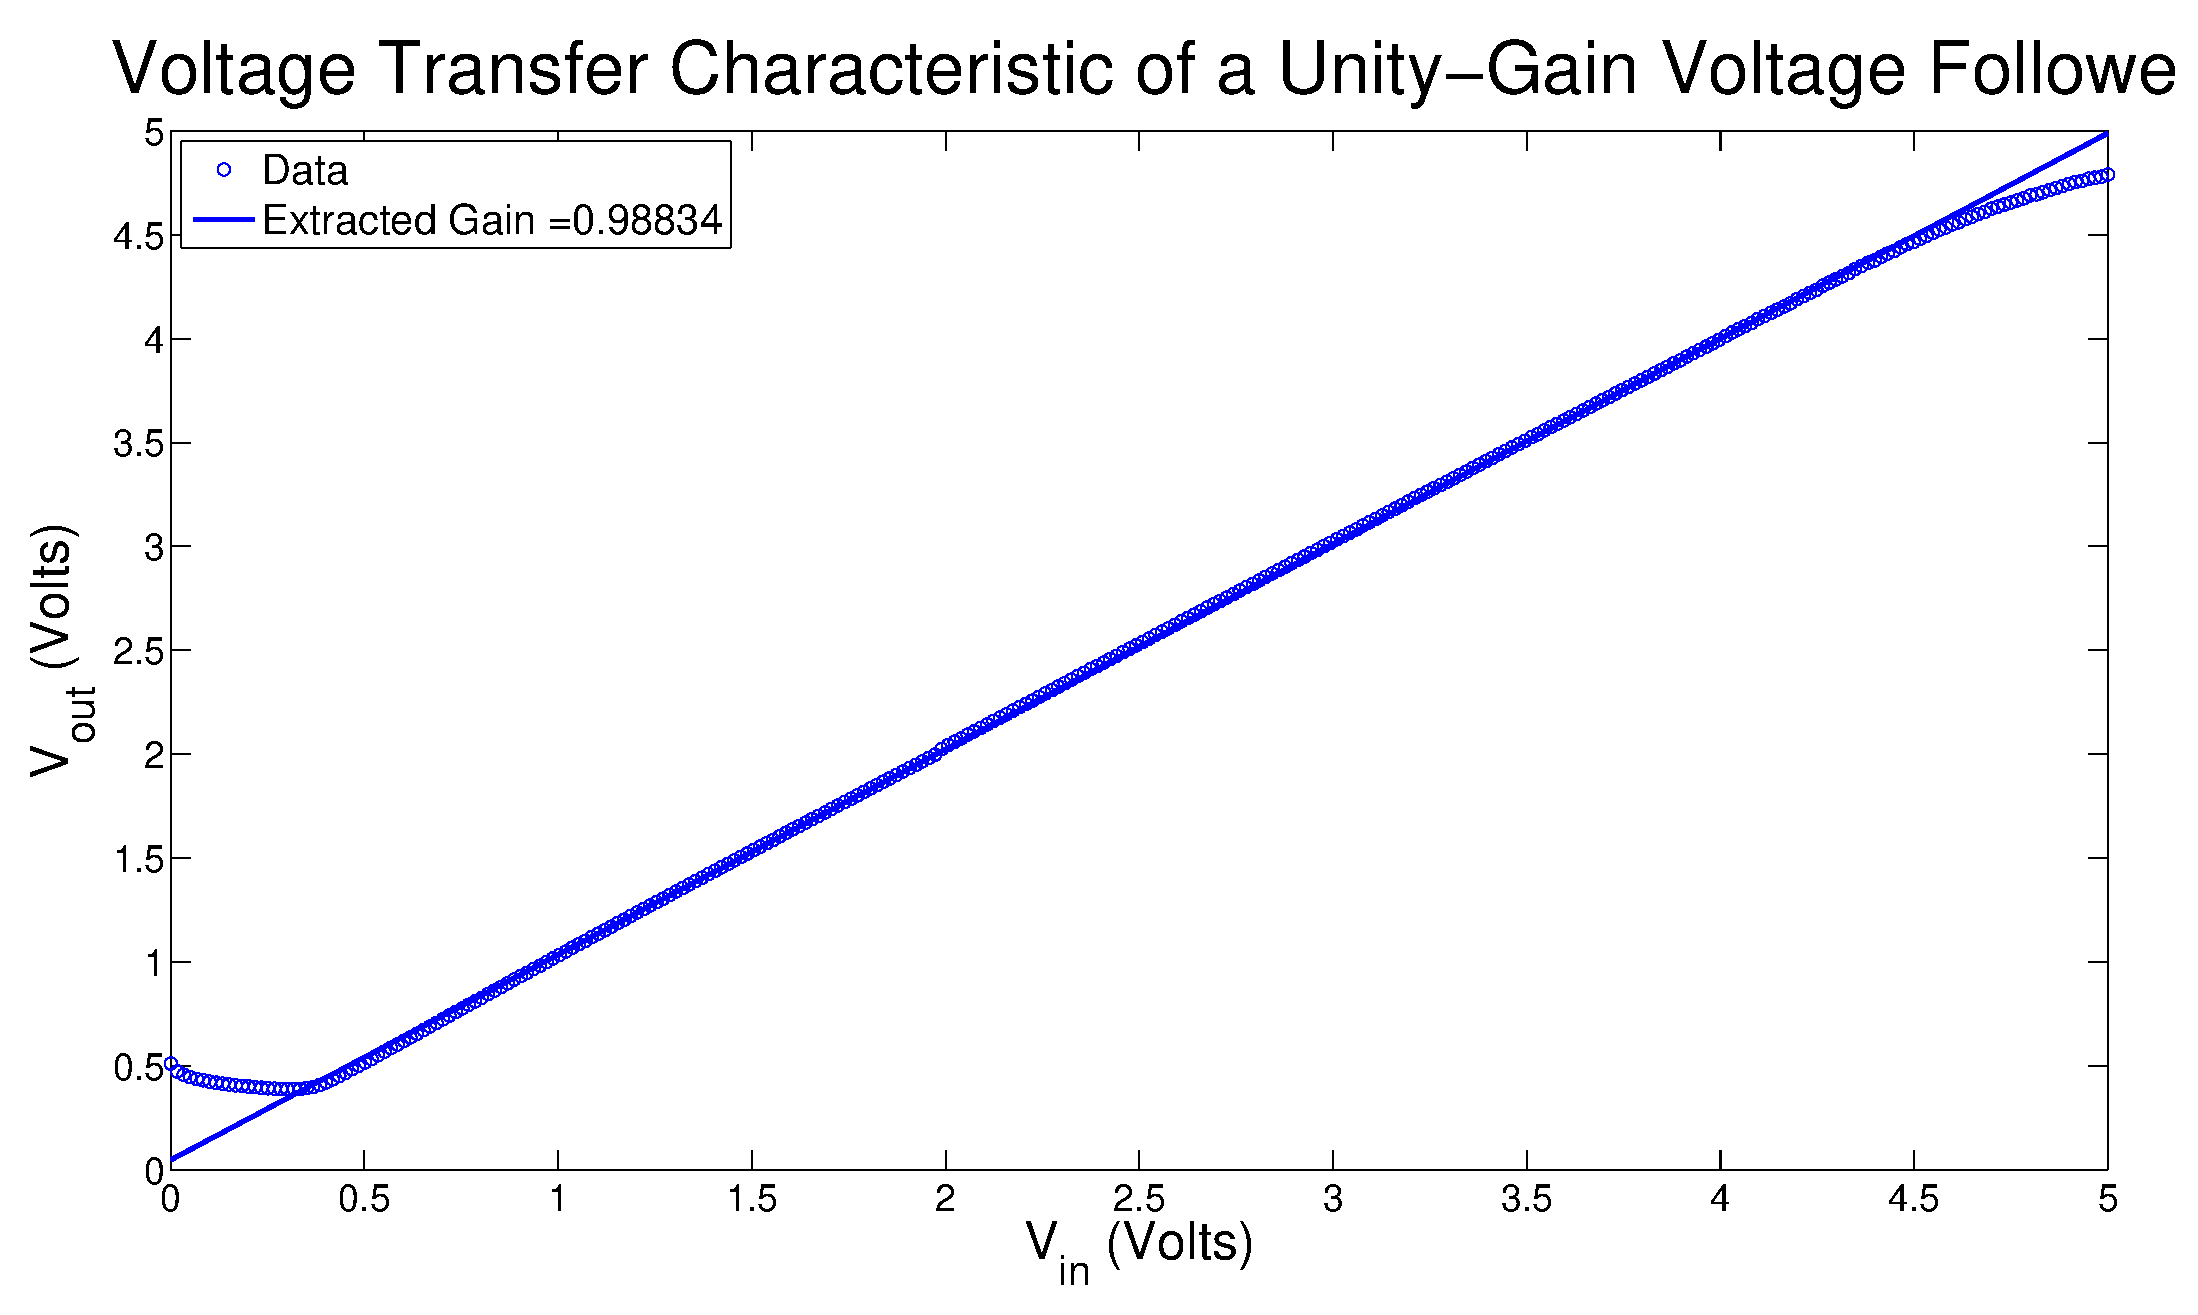
\includegraphics[width=\linewidth]{../Figures/Exp3P1.eps}
\caption{Something descriptive..}
\label{fig:exp3p1}
\end{figure}

So we connected the output and the input of the differential amplifier and measured \Vout as we swept \Vin from ground to \Vdd. The results are shown in figure \ref{fig:exp3p1}, in addition to a line fitted to the linear region of the voltage transfer characteristic. We extract the slope of this line and found that the actual gain of the follower was 0.98834, very close to the anticipated gain of 1. The slight deviation, a little over 1\%, can likely be attributed to experimental error. The behavior of the circuit for small values of \Vin can likely be attributed to both \Mone and \Mtwo operating in weak inversion, which causes \Iout to be the difference between their very small leakage currents, which therefore causes \Vout to change little for $0 \leq V_{in} \leq \approx 0.5 V.$

We can also see that the near-unity gain between \Vout and \Vin breaks down for values of \Vin near \Vdd. This could be due to the bias transistor not passing as much current as \Mone can pass, so as the gate voltage of \Mone increases, \Ib increases less than expected, which causes \Vout to increase less than linearly.

Since we expected $\frac{V_{out}}{V_{in}} \approx 1$, we next looked at the offset voltage of the bias transistor ($V_{out} - V_{in}$) in order to gain further insight into how our unity-gain buffer behaves compared to the ideal form of the circuit, which would have an offset voltage of 0.

\begin{figure}[H]
\centering
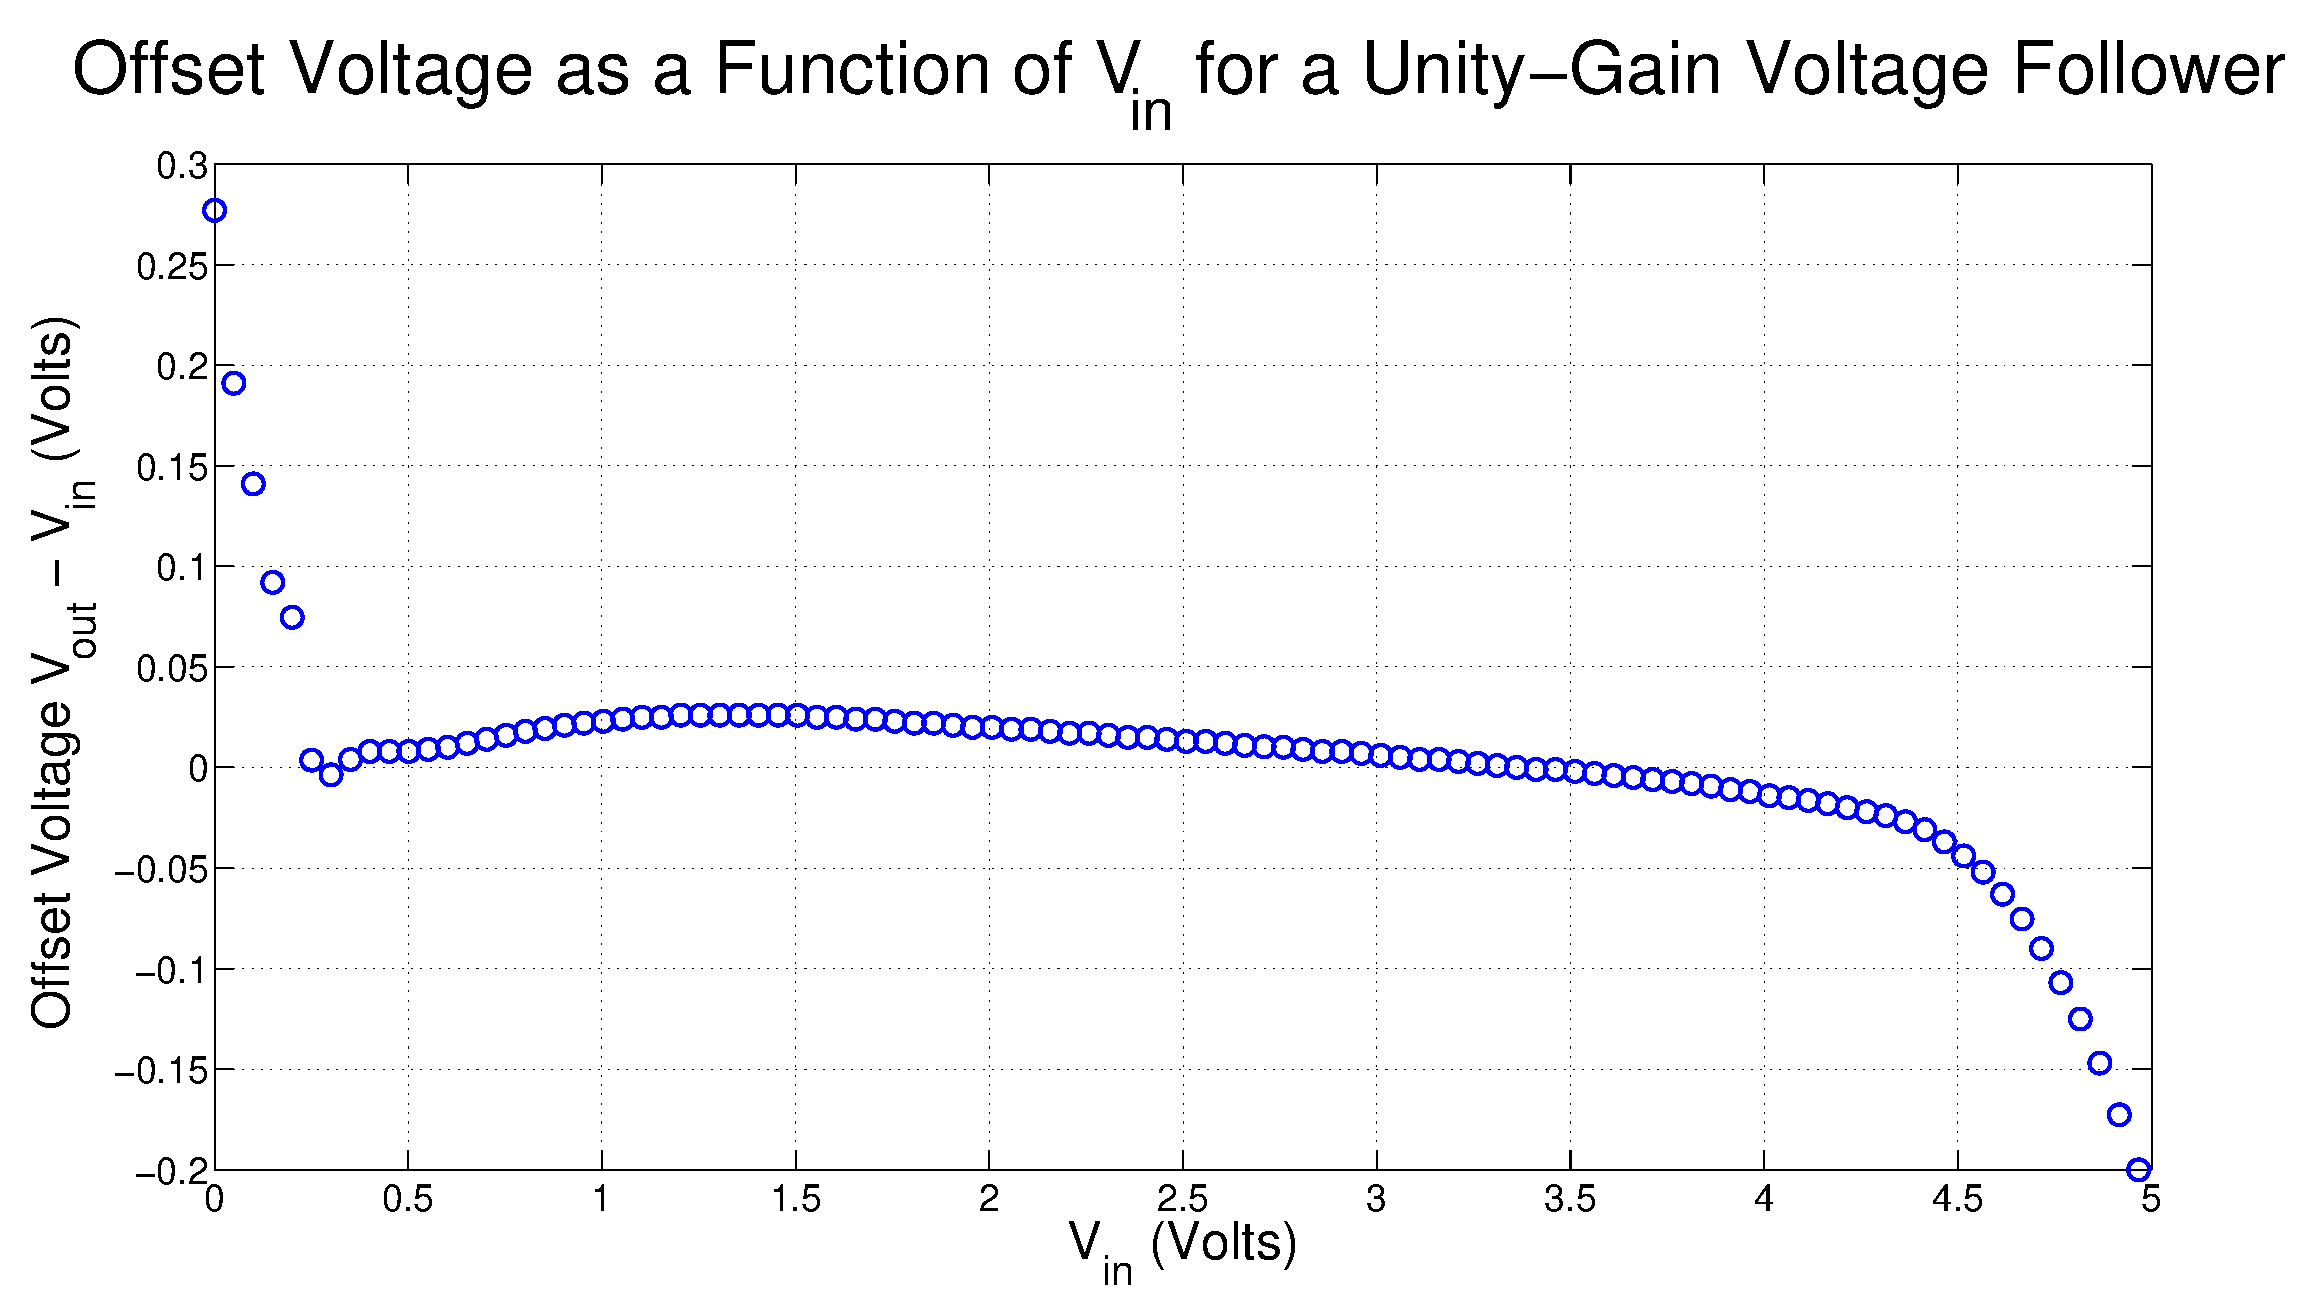
\includegraphics[width=\linewidth]{../Figures/Exp3P2.eps}
\caption{Something descriptive..}
\label{fig:exp3p2}
\end{figure}

Figure \ref{fig:exp2p2} shows the offset voltage of the buffer as a function of \Vin, and some interesting trends appear. We again see large deviations from the theoretical ideal at values of \Vin near ground and near \Vdd, which could be explained by leakage current and a saturated \Mb, respectively.

The trend in the middle of the data seems to take two forms: for $0.5 < V_{in} < 1.5$, the offset voltage has a small positive slope, but for $1.5 < V_{in} < 4.5$, this slope becomes negative, and the trend is far more linear. Generally, however, the offset voltage hovers around 0, and deviates by about $\pm 0.02 V$ throughout the region of linear operation that we saw in figure \ref{fig:exp3p1}. 


\end{document}